\documentclass{beamer}
\usetheme{Berkeley}
\title{Matrix Project}
\subtitle{EE1390: Intro to AI and ML}
\author{Tejas Meshram\inst{1} \and Abhishek K. Singh\inst{2}}
\institute[IIT Hyderabad]
{
  \inst{1}%
  ME17BTECH11046
  \and
  \inst{2}%
  EP17BTECH11020
}
\date{\today}
\subject{Analysis}
\AtBeginSubsection[]
{
  \begin{frame}<beamer>{Analysis}
    \tableofcontents[currentsection,currentsubsection]
  \end{frame}
}

\begin{document}

\begin{frame}
  \titlepage
\end{frame}

\begin{frame}{Problem Solving Strategy}
  \tableofcontents
\end{frame}

\section{Graphical Verification}

\subsection{}

\begin{frame}{Matrix problem in coordinate geometry}{From JEE Main 2018}
  \begin{itemize}
\item If $\bf \beta$ is one of the angles between the normals of the ellipse $\textbf{X}^TV\textbf{X} = 9$ at
the points
$\begin{pmatrix}
           3 \cos\theta\\
           \sqrt{3}\sin\theta\\
\end{pmatrix}$,
$\begin{pmatrix}
           -3 \sin\theta \\
           \sqrt{3}\cos\theta \\
\end{pmatrix}$;
$\theta \in (0, \frac{\pi}{2})$, 
$V = \begin{bmatrix}
           1 & 0\\
           0 & 3 \\
\end{bmatrix}$;
then $\frac{2\cot\textbf{\beta}}{\sin 2\theta}$ is equal to..
  \end{itemize}
\end{frame}

\subsection{Using Python}

\begin{frame}{Graphical Analysis}
\begin{block}{}
Using python libraries, the following graphs are plotted
\item  1.Normal to ellipse at point\textbf{ A }and  \textbf{B} intersecting at \textbf{N}
\item  2.Polar graph of $\beta$ for given value of $\theta$
\item  3.Graph of 2$\cot \beta$  Vs $\sin 2\theta$  
\\
ref: \url{https://github.com/tejasmeshram99/EE1390}
\end{block}
\end{frame}
\begin{frame}{Figure 1}
At $\theta =\frac{\pi}{4}$ 

\centering
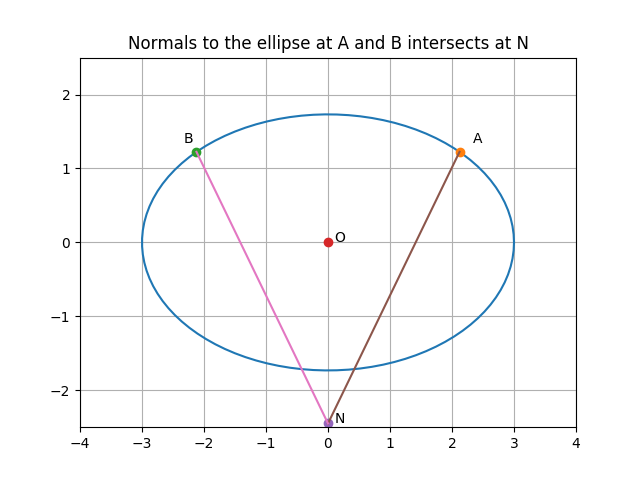
\includegraphics[scale=0.6]{preambule/normals_4.png}
\end{frame}
\begin{frame}{Figure 2}
At $\theta =\frac{\pi}{4}$ 

\centering
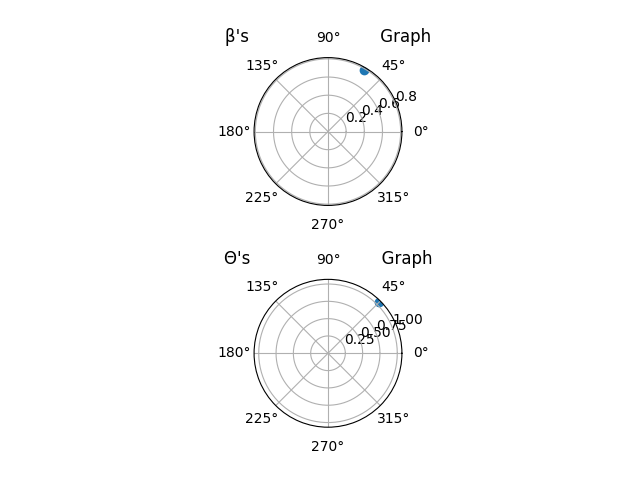
\includegraphics[scale=0.6]{preambule/angles_4.png}
\end{frame}
\begin{frame}{Figure 3}
At $\theta =\frac{\pi}{4}$ point is $\begin{pmatrix}1& 2/\sqrt{3}\end{pmatrix}$.

\centering
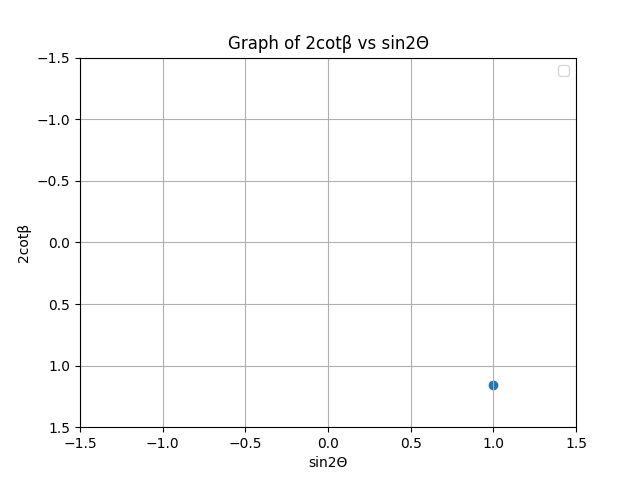
\includegraphics[scale=0.6]{preambule/points_4.png}
\end{frame}
\begin{frame}{Graphical Analysis}
\begin{block}{Results}
{\Large For different values of $\theta \in (0, \pi/2)$, the slope of  $2\cot\beta$ vs $\sin2\theta$ 
turns out
to be \alert{$\frac{2}{\sqrt{3}}$ } or \alert{1.155},
which is independent of $\theta$ and $\beta$.}
\end{block}
\end{frame}

\section{Theoretical Computation}
\subsection{Using Matrix}

\begin{frame}{Solution}
  \begin{itemize}
\item<1->
We've equation of the ellipse $\textbf{X}^TV\textbf{X} = 9$ and two points \textbf{A} and \textbf{B}.
Where,
$V = \begin{bmatrix}
           1 & 0 \\
           0 & 3 \\
  \end{bmatrix}$, 
$\textbf{A}= \begin{pmatrix}
           3 \cos\theta\\
           \sqrt{3}\sin\theta \\
  \end{pmatrix}$
   and $\textbf{B}=\begin{pmatrix}
           -3 \sin\theta \\
           \sqrt{3}\cos\theta \\
  \end{pmatrix}$.
\item<2->
Equation of tangents at points \textbf{A} and \textbf{B} can be written as
$\textbf{A}^TV\textbf{X} = 9$ 
\implies $\textbf{{n}_1}^T\textbf{X} = 9$$ \\
where, \textbf{{n}_1}^T =\textbf{A}^TV=\begin{bmatrix}
           3\cos\theta&3\sqrt{3}\sin\theta
\end{bmatrix}$
\item<3->
$\textbf{B}^TV\textbf{X} = 9$ 
\implies $\textbf{{n}_2}^T\textbf{X} = 9$$\\
where, \textbf{{n}_2}^T =\textbf{B}^TV=\begin{bmatrix}
           -3\sin\theta&3\sqrt{3}\cos\theta
\end{bmatrix}$
  \end{itemize}
\end{frame}

\begin{frame}{Solution(Cont'd)}
  \begin{itemize}
\item<1->
The angle between normal vectors ${n}_1, {n}_2$ is
$\beta$, $0\leq\beta\leq\pi$
\\
${\Large \cos\beta = \frac{{n}_1^T{n}_2}{\|{n}_1\|\|{n}_2\|}}$;
%\item Using ${n}_1^T{n}_2  =9\sin 2\theta$,  $\|{n}_1\|\|{n}_2\| = 9\left(1+\sin ^2\theta)\right  9\left(1+\cos ^2\theta)\right$
            \item<2->
\\
{\Large $\cot\beta = \frac{{n}_1^T{n}_2}{\sqrt{\left(\|{n}_1\|\|{n}_2\|\right)^2-\left({n}_1^T{n}_2\right)^2}}$
= $\frac{\sin2\theta}{\sqrt{3}}$}
\item<3->
Therefore,
{\LARGE $\frac{2\cot\beta}{\sin2\theta} = \frac{2}{\sqrt{3}}$}.
\end{itemize}
\end{frame}


\appendix\textbf{}
\section<presentation>*{\appendixname}
\subsection<presentation>*{Reference}

\begin{frame}[allowframebreaks]
  \frametitle<presentation>{References}
    
  \begin{thebibliography}{10}
 
  \beamertemplatearticlebibitems

  \bibitem{Sharma}
    G. V. V. ~Sharma.
    \newblock EE1390
    \newblock {\em Introduction to AI and ML}, Spring,
    2019.\\
    \url{github.com/gadepall/school/tree/master/linalg}
\beamertemplatearticlebibitems

  \bibitem{Online}
    Latex Beamer
    \url{https://www.overleaf.com/learn/latex/Beamer} \url{http://detexify.kirelabs.org/classify.html}
    
  \end{thebibliography}
\end{frame}
\item {\HUGE Thanks!!}
\item Mail IDs : \href{mailto:ep17btech11020@iith.ac.in}{Abhishek},\href{mailto:me17btech11046@iith.ac.in}{Tejas}.
\end{document}
